% Faraday/Lenz: zunehmender Fluss durch A induziert E entgegen der Orientierung von \partial A
% Gemeinsamer Stil für alle Abbildungen (TikZ -> SVG, siehe figures/build.mjs).
%
% Farben sind Platzhalter ("Sentinels"): build.mjs ersetzt sie im SVG durch
% CSS-Variablen, damit die Abbildungen im hellen und dunklen Modus passen.
% Andere Farben (auch schwarz/weiß) bricht der Build mit Fehler ab.
%
%   fg    Linien, Beschriftung          -> --dark
%   mu    Hilfslinien, Achsen, Maße      -> --gray
%   acc   das eine Konzept der Abbildung -> --secondary (Lime/Oliv)
%   blue  zweite Größe, negative Ladung  -> --fig-blue
%   warm  dritte Größe, positive Ladung  -> --fig-warm
%   bg    Seitenhintergrund (Aussparen)  -> --light
%
% Kein \clip verwenden: pdftocairo macht daraus Clip-Gruppen, in denen exakt
% waagerechte/senkrechte Linien verschwinden. Berechnete Kurven schneidet
% gen/*.py selbst am Rahmen ab.
\documentclass[tikz,border=3pt]{standalone}
\usepackage{amsmath,amssymb,bm}
% Text serifenlos wie die Seite, Mathe in Computer Modern wie KaTeX
\renewcommand{\familydefault}{\sfdefault}
\usetikzlibrary{arrows.meta,calc,decorations.markings,patterns,3d,positioning,angles,quotes}

\definecolor{fg}{RGB}{1,2,3}
\definecolor{mu}{RGB}{4,5,6}
\definecolor{acc}{RGB}{7,8,9}
\definecolor{blue}{RGB}{10,11,12}
\definecolor{warm}{RGB}{13,14,15}
\definecolor{bg}{RGB}{16,17,18}

% Vektoren wie auf der Website (KaTeX \mathbf)
\newcommand{\vv}[1]{\mathbf{#1}}

\tikzset{
  every picture/.style={fg, line width=0.8pt, line cap=round, line join=round,
    >={Stealth[length=5.5pt,width=4.4pt]}},
  every node/.style={font=\small},
  % Linientypen
  main/.style={line width=0.9pt},
  thin/.style={line width=0.5pt},
  aux/.style={mu, line width=0.5pt, dash pattern=on 2.5pt off 2pt},
  axis/.style={mu, line width=0.6pt, ->},
  vec/.style={line width=1.1pt, ->},
  field/.style={line width=0.7pt, postaction={decorate},
    decoration={markings, mark=at position #1 with {\arrow{Stealth[length=4.5pt,width=3.6pt]}}}},
  field/.default=0.5,
  % Flächen
  soft/.style={fill=#1, fill opacity=0.14},
  soft/.default=acc,
  % Ladungen
  qpos/.style={circle, fill=warm, inner sep=0pt, minimum size=9pt,
    path picture={\draw[bg, line width=0.9pt] ($(path picture bounding box.center)+(-2pt,0)$) -- +(4pt,0)
      ($(path picture bounding box.center)+(0,-2pt)$) -- +(0,4pt);}},
  qneg/.style={circle, fill=blue, inner sep=0pt, minimum size=9pt,
    path picture={\draw[bg, line width=0.9pt] ($(path picture bounding box.center)+(-2pt,0)$) -- +(4pt,0);}},
  dot/.style={circle, fill=fg, inner sep=0pt, minimum size=3pt},
  % Beschriftung mit Aussparung, damit Linien den Text nicht kreuzen
  lbl/.style={fill=bg, inner sep=1.5pt},
  % Icons: kräftigere Linien, keine Schrift
  icon/.style={line width=1.6pt, >={Stealth[length=6pt,width=5pt]}},
}

\begin{document}
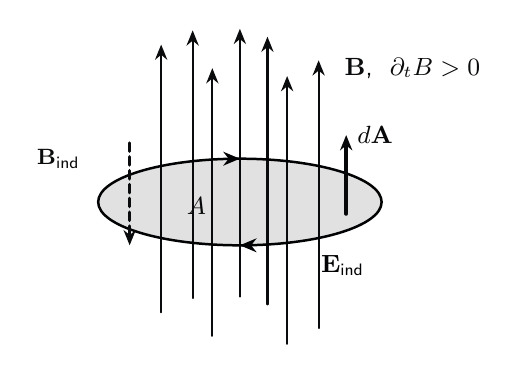
\begin{tikzpicture}[yscale=1]
  \def\R{1.8} \def\h{0.55} % Ellipse: Halbachsen R (x) und h (Tiefe)
  % B-Feldlinien (hinter der Fläche beginnen)
  \foreach \x/\y in {-1.0/0.1, -0.35/-0.2, 0.35/0.2, 1.0/-0.1, 0/0.3, -0.6/0.28, 0.6/-0.3} {
    \draw[blue, line width=0.8pt, ->] (\x,\y-1.5) -- (\x,\y+1.9);
  }
  % Fläche A mit Rand; Rückseite zuerst
  \fill[acc, fill opacity=0.12] (0,0) ellipse ({\R} and {\h});
  % Blick von vorn-oben: vorderer Rand = unten im Bild. Positive Orientierung zu dA (nach oben)
  % ist von oben gesehen gegen den Uhrzeigersinn, vorne also nach rechts. Lenz: E_ind läuft
  % umgekehrt, also Bogen im Uhrzeigersinn (360 -> 0): vorne nach links, hinten nach rechts.
  \draw[main, postaction={decorate}, decoration={markings,
      mark=at position 0.25 with {\arrow{Stealth[length=6pt,width=5pt]}},
      mark=at position 0.75 with {\arrow{Stealth[length=6pt,width=5pt]}}}]
    (\R,0) arc[start angle=360, end angle=0, x radius=\R, y radius=\h];
  % Normale dA
  \draw[vec, acc, line width=1.4pt] (1.35,-0.15) -- ++(0,1.0) node[anchor=west] {$d\vv A$};
  % induziertes Gegenfeld
  \draw[blue, line width=1.2pt, dash pattern=on 3pt off 2pt, ->] (-1.4,0.75) -- (-1.4,-0.55);
  \node[blue, anchor=east, font=\footnotesize] at (-1.9,0.55) {$\vv B_{\text{ind}}$};
  \node[blue, anchor=west] at (1.2,1.7) {$\vv B$, \ $\partial_t B>0$};
  \node[anchor=north west] at (0.9,-0.55) {$\vv E_{\text{ind}}$};
  \node[acc] at (-0.55,-0.05) {$A$};
\end{tikzpicture}
\end{document}
